\documentclass{article}
\usepackage[utf8]{inputenc}
\usepackage{graphicx}

\title{BDSA Exercise 1}
\author{guho }
\date{September 2021}

\begin{document}

\maketitle

\section{Main function}

In the flowchart shown below, it is visualizing what happens in the main function, where it gets an input, and does some error handling before it sends it off to the IsLeapYear function. It checks if it is able to make it into an integer first, and then checks if the year given is 1582 or higher. If it passes the two checks, it will send the input to the IsLeapYear function, and gets returned a true or false, which makes it print either a yay or nay.

\begin{figure}[ht]
    \centering
    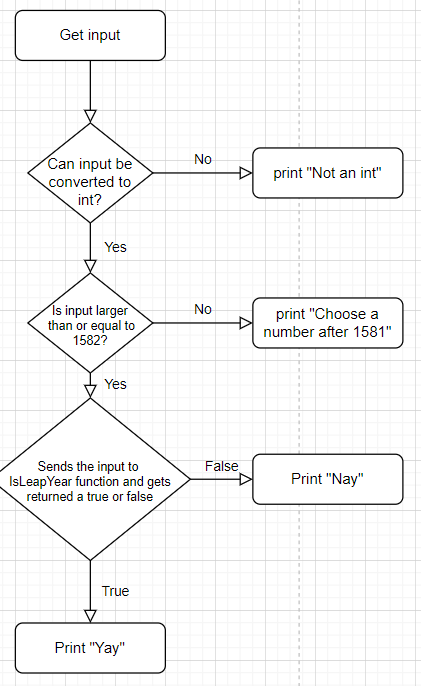
\includegraphics[scale=0.6]{Pictures/main flowchart.PNG}
    \caption{Main flowchart}
    \label{fig:main}
\end{figure}

\section{IsLeapYear function}

In this flowchart, it describes what happens when it gets the input from main, and checks if it is a leap year or not. First it checks if the year is divisible by 400, then it checks if the year is divisible by 100, and in the end checks if the year is divisible by 4. Depending on what check it succeeds or doesn't succeed it will return a true or false to the main function.

\begin{figure}[ht]
    \centering
    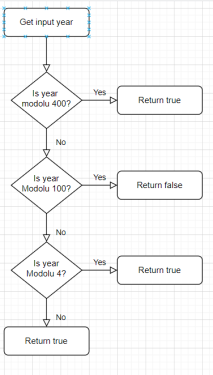
\includegraphics[scale=0.6]{Pictures/IsLeapYear flowchart.png}
    \caption{IsLeapYear flowchart}
    \label{fig:IsLeapYear}
\end{figure}

\end{document}
